\section{Anwendungsprotokolle}

\subsection{HTTP}

\begin{defi}{HTTP}
    Das \emph{Hypertext Transfer Protocol (HTTP)} ist ein Protokoll zur Übertragung von Daten auf der Anwendungsschicht über ein Rechnernetz.
    Es wird hauptsächlich eingesetzt, um Webseiten (Hypertext-Dokumente) aus dem World Wide Web (WWW) in einen Webbrowser zu laden.
    Es ist jedoch nicht prinzipiell darauf beschränkt und auch als allgemeines Dateiübertragungsprotokoll sehr verbreitet.

    HTTP ist ein zustandsloses Protokoll (Informationen aus früheren Anforderungen gehen verloren).
    Ein zuverlässiges Mitführen von Sitzungsdaten kann erst auf der Anwendungsschicht durch eine Sitzung über einen Sitzungsbezeichner implementiert werden.

    Über Cookies in den Header-Informationen können aber Anwendungen realisiert werden, die Statusinformationen (Benutzereinträge, Warenkörbe) zuordnen können.
    Dadurch werden Anwendungen möglich, die Status- beziehungsweise Sitzungseigenschaften erfordern.
    Auch eine Benutzerauthentifizierung ist möglich.

    Normalerweise kann die Information, die über HTTP übertragen wird, auf allen Rechnern und Routern gelesen werden, die im Netzwerk durchlaufen werden.
    Über HTTPS jedoch kann die Übertragung verschlüsselt erfolgen.
\end{defi}

\begin{defi}{HTTP-Anfragen und -Methoden}
    Die Kommunikationseinheiten in HTTP zwischen Client und Server werden als Nachrichten bezeichnet, von denen es zwei unterschiedliche Arten gibt: die Anfrage (\emph{Request}) vom Client an den Server und die Antwort (\emph{Response}) als Reaktion darauf vom Server zum Client.

    Jede Nachricht besteht dabei aus zwei Teilen, dem \emph{Message Header} bzw. \emph{HTTP-Header} und dem \emph{Message Body}.

    Der Message Header enthält Informationen über den Message Body wie etwa verwendete Kodierungen oder den Inhaltstyp, damit dieser vom Empfänger korrekt interpretiert werden kann.

    Der Message Body enthält schließlich die Nutzdaten.

    HTTP-Anfragemethoden sind:
    \begin{itemize}
        \item \texttt{GET} fordert eine Ressource an.
        \item \texttt{POST} schickt Daten zur weiteren Verarbeitung zum Server.
        \item \texttt{HEAD} weist den Server an, die gleichen HTTP-Header wie bei \texttt{GET}, nicht jedoch den Nachrichtenrumpf mit dem eigentlichen Dokumentinhalt zu senden.
        \item \texttt{PUT} dient dazu, eine Ressource unter Angabe des Ziel-URIs auf einen Webserver hochzuladen.
        \item \texttt{PATCH} ändert ein bestehendes Dokument ohne dieses wie bei PUT vollständig zu ersetzen.
        \item \texttt{DELETE} löscht die angegebene Ressource auf dem Server.
        \item \texttt{TRACE} liefert die Anfrage so zurück, wie der Server sie empfangen hat.
        \item \texttt{OPTIONS} liefert eine Liste der vom Server unterstützten Methoden und Merkmale.
        \item \texttt{CONNECT} wird von Proxyservern implementiert, die in der Lage sind, SSL-Tunnel zur Verfügung zu stellen.
    \end{itemize}
\end{defi}

\begin{defi}{HTTP-Request}
    \centering
    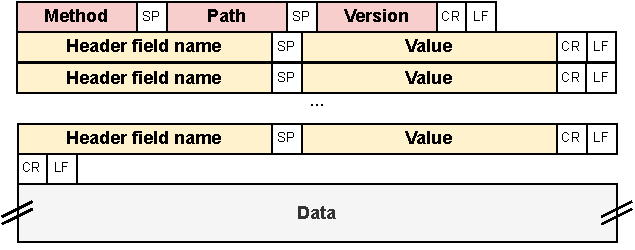
\includegraphics[width=.7\textwidth]{includes/figures/defi_http_request_header.pdf}
\end{defi}

\begin{defi}{HTTP-Response}
    \centering
    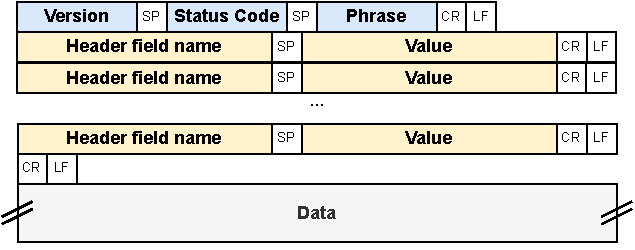
\includegraphics[width=.7\textwidth]{includes/figures/defi_http_response_header.pdf}
\end{defi}

\begin{example}{HTTP-GET-Request}
    \centering
    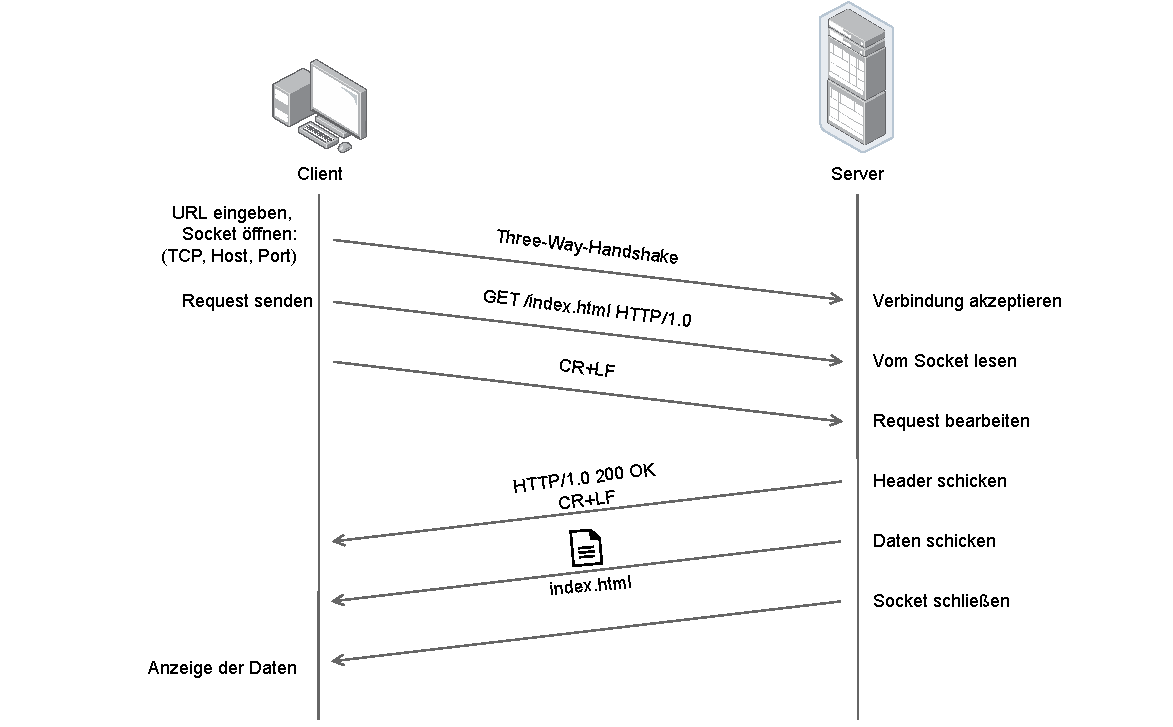
\includegraphics[width=.9\textwidth]{includes/figures/defi_http_get.pdf}
\end{example}

\subsection{MIME}

\begin{defi}{MIME}
    Die \emph{Multipurpose Internet Mail Extensions (MIME)} sind Erweiterungen des Internetstandards \href{https://datatracker.ietf.org/doc/html/rfc822}{RFC 822}, der das Datenformat von E-Mails definiert. Dieser sieht nur den American Standard Code for Information Interchange (ASCII) vor.

    Die MIME schaffen Kompatibilität für zusätzliche Zeichen wie Umlaute sowie für Multimedia (etwa bei Mail-Anhängen).

    Darüber hinaus findet MIME Anwendung bei der Deklaration von Inhalten in verschiedenen Internetprotokollen wie etwa HTTP sowie bei Desktop-Umgebungen wie KDE, Gnome, Xfce oder Aqua\footnote{Aqua ist die grafische Benutzeroberfläche von macOS.}.

    Der MIME-Header besteht aus:
    \begin{itemize}
        \item \texttt{MIME-Version}:
              \begin{itemize}
                  \item Damit ein MIME-Dokument mit RFC 2045 konform ist, muss sich dieses Feld im Header der höchsten Ebene befinden und den Wert \texttt{1.0} haben.
              \end{itemize}
        \item \texttt{Content-Type}:
              \begin{itemize}
                  \item \texttt{Content-Type} hat standardmäßig den Wert \texttt{text/plain}.
                  \item \texttt{Content-Type} definiert den Datentyp in jedem Nachrichtenteil als \texttt{Typ/Subtyp}.
                  \item Der MIME-Parser akzeptiert die meisten Werte für \texttt{Content-Type} und speichert sie in der logischen Baumstruktur.
              \end{itemize}
        \item \texttt{Content-Transfer-Encoding}:
              \begin{itemize}
                  \item Optional.
              \end{itemize}
        \item \texttt{Content-ID}:
              \begin{itemize}
                  \item Optional.
                  \item Mit diesem Feld können Nachrichtenteile mit einer Inhalts-ID versehen und so von anderen Teilen der Nachricht referenziert werden.
              \end{itemize}
        \item \texttt{Content-Description}:
              \begin{itemize}
                  \item Optional.
                  \item Dieses Feld kann Beschreibungen zu Nachrichtenteilen enthalten.
              \end{itemize}
    \end{itemize}
\end{defi}

\begin{defi}{MIME Content-Types}
    Die wichtigsten Typen sind unter Anderem:

    \begin{tabularx}{\textwidth}{|T|X|}
        \hline
        Content-Type             & Anwendung                                                                                                  \\
        \hline
        \hline
        text/plain               & Allgemein für eine typische Mail oder Newsnachricht verwendet.                                             \\
        \hline
        text/xml                 & Allgemein in Verbindung mit SwA-Nachrichten (SOAP with Attachments) verwendet.                             \\
        \hline
        application/octet-stream & Verwendet, wenn der Typ der Nachricht unbekannt ist und enthält beliebige Daten als Bytes.                 \\
        \hline
        application/xml          & Für anwendungsspezifische XML-Daten verwendet.                                                             \\
        \hline
        x-type                   & Für vom Standard abweichende Inhaltstypen verwendet. Muss mit \texttt{x-} beginnen.                        \\
        \hline
        image/jpeg               & Für Bilder verwendet. \texttt{image/jpeg} und \texttt{image/gif} sind allgemein gebräuchliche Bildformate. \\
        \hline
        multipart/related        & Für mehrere zusammengehörige Teile in einer Nachricht verwendet, insbesondere mit SwA.                     \\
        \hline
        multipart/signed         & Für mehrere zusammengehörige Teile in einer Nachricht, einschließlich Signatur, verwendet.                 \\
        \hline
        multipart/mixed          & Für mehrere unabhängige Teile in einer Nachricht verwendet.                                                \\
        \hline
    \end{tabularx}
\end{defi}

\subsection{Sichere Protokolle}

\begin{defi}{HTTPS}
    \emph{Hypertext Transfer Protocol Secure (HTTPS)}  ist ein Kommunikationsprotokoll im World Wide Web, mit dem Daten abhörsicher übertragen werden können. Es stellt eine Transportverschlüsselung dar.

    HTTPS wird zur Herstellung von Vertraulichkeit und Integrität in der Kommunikation zwischen Webserver und Webbrowser (Client) im World Wide Web verwendet.
    Dies wird unter anderem durch Verschlüsselung und Authentifizierung erreicht.

    Ohne Verschlüsselung sind Daten, die über das Internet übertragen werden, für jeden, der Zugang zum entsprechenden Netz hat, als Klartext lesbar.
    Mit der zunehmenden Verbreitung von offenen (d. h. unverschlüsselten) WLANs nimmt die Bedeutung von HTTPS zu, weil damit die Inhalte unabhängig vom Netz verschlüsselt werden können.

    Die Authentifizierung dient dazu, dass beide Seiten der Verbindung beim Aufbau der Kommunikation die Identität des Verbindungspartners überprüfen können.
    Dadurch sollen Man-in-the-Middle-Angriffe und teilweise auch Phishing verhindert werden.

    Syntaktisch ist HTTPS identisch mit dem Schema für HTTP, die zusätzliche Verschlüsselung der Daten geschieht mittels SSL/TLS: Unter Verwendung des SSL-Handshake-Protokolls findet zunächst eine geschützte Identifikation und Authentifizierung der Kommunikationspartner statt. Anschließend wird mit Hilfe asymmetrischer Verschlüsselung oder des Diffie-Hellman-Schlüsselaustauschs ein gemeinsamer symmetrischer Sitzungsschlüssel ausgetauscht.
    Dieser wird schließlich zur Verschlüsselung der Nutzdaten verwendet.
\end{defi}

\begin{defi}{SSL/TLS}
    \emph{Transport Layer Security (TLS)}, auch bekannt unter der Vorgängerbezeichnung \emph{Secure Sockets Layer (SSL)}, ist ein Verschlüsselungsprotokoll zur sicheren Datenübertragung im Internet.

    TLS besteht aus den beiden Hauptkomponenten \emph{TLS Handshake} und \emph{TLS Record}.

    Im OSI-Modell ist TLS in Schicht 5 (der Sitzungsschicht) angeordnet.
    Im TCP/IP-Modell ist TLS oberhalb der Transportschicht (zum Beispiel TCP) und unterhalb Anwendungsprotokollen wie HTTP oder SMTP angesiedelt.
\end{defi}

\begin{defi}{TLS Handshake Protocol}
    Das \emph{TLS Handshake Protocol} baut auf dem TLS Record Protocol auf und erfüllt die folgenden Funktionen, noch bevor die ersten Bits des Anwendungsdatenstromes ausgetauscht wurden:
    \begin{itemize}
        \item Aushandeln zu benutzender kryptografischer Algorithmen und Schlüssel. TLS unterstützt auch eine unverschlüsselte Übertragung.
        \item Identifikation und Authentifizierung der Kommunikationspartner auf Basis asymmetrischer Verschlüsselungsverfahren und Public-Key-Kryptografie.\footnote{Dieser Schritt ist optional eine Zwei-Wege-Authentifizierung (in diesem Fall wird manchmal von mutual TLS gesprochen), für gewöhnlich authentifiziert sich aber nur der Server gegenüber dem Client.}
    \end{itemize}

    Insgesamt besteht der TLS Handshake aus vier Phasen:
    \begin{enumerate}
        \item Der Client schickt zum Server ein \texttt{ClientHello}, und der Server antwortet dem Client mit einem \texttt{ServerHello}. Die Parameter der Nachrichten sind:
              \begin{itemize}
                  \item die Version (die höchste vom Client unterstützte TLS-Protokoll-Version)
                  \item eine 32 Byte lange Zufallsinformation
                  \item eine Session-ID
              \end{itemize}
        \item Der Server identifiziert sich gegenüber dem Client.
              \begin{itemize}
                  \item Hierzu wird per Certificate ein \emph{X.509-Zertifikat} an den Client geschickt, gefolgt von einem \texttt{CertificateVerify} (in einigen TLS Versionen).
                  \item Die \texttt{CertificateVerify} Nachricht enthält eine Unterschrift von zuvor ausgetauschten Nachrichten.
                  \item Der Client prüft das Zertifikat und die Unterschrift. Bei Misserfolg bricht der Client die Verbindung ab.
                  \item Außerdem kann der Server optional per \texttt{CertificateRequest} ein Zertifikat zur Client-Authentifizierung anfordern.
              \end{itemize}
        \item Das zuvor erhaltene Server-Zertifikat enthält den öffentlichen Schlüssel des Servers. Es wird ein Diffie-Hellman-Schlüsselaustausch durchgeführt, um ein gemeinsames \emph{pre-master-secret} zu generieren.
        \item Diese Phase schließt den Handshake ab. Aus dem vorhandenen pre-master-secret kann das \emph{master secret} abgeleitet werden, das einen einmaligen \emph{Sitzungsschlüssel (Session Key)} darstellt.
              \begin{itemize}
                  \item Aus dem master secret werden wiederum \emph{Schlüssel} abgeleitet, die zum Ver- und Entschlüsseln der Daten sowie für die Integritätsprüfung verwendet werden.
                  \item Die Nachrichten, die die Kommunikationspartner sich nun gegenseitig zusenden, werden nur noch verschlüsselt übertragen.
              \end{itemize}
    \end{enumerate}
\end{defi}

\begin{defi}{TLS Record Protocol}
    Das \emph{TLS Record Protocol} dient zur Absicherung der Verbindung.

    Es setzt direkt auf der Transportschicht auf und bietet zwei verschiedene Dienste, die einzeln oder gemeinsam genutzt werden können:
    \begin{itemize}
        \item Ende-zu-Ende-Verschlüsselung mittels symmetrischer Algorithmen. Der verwendete Schlüssel wird dabei im Voraus über ein weiteres Protokoll (zum Beispiel das TLS Handshake Protocol) ausgehandelt und kann nur einmal für die jeweilige Verbindung verwendet werden.
        \item Sicherung der Nachrichten-Integrität und Authentizität durch einen Message Authentication Code (MAC).
    \end{itemize}
\end{defi}

\begin{bonus}{X.509 Zertifikat}
    \emph{X.509} ist ein Standard für eine Public-Key-Infrastruktur zum Erstellen digitaler Zertifikate.

    In der elektronischen Kommunikation finden X.509-Zertifikate Anwendung bei den TLS-Versionen diverser Übertragungsprotokolle, wie z. B. beim Abruf von Web-Seiten mit HTTPS oder zum Unterschreiben und Verschlüsseln von E-Mails nach dem S/MIME-Standard.

    Struktur eines X.509-v3-Zertifikats:
    \begin{itemize}
        \item Zertifikat
              \begin{itemize}
                  \item Version
                  \item Seriennummer
                  \item Algorithmen-ID
                  \item Aussteller
                  \item Gültigkeit
                        \begin{itemize}
                            \item von
                            \item bis
                        \end{itemize}
                  \item Zertifikatinhaber
                  \item Zertifikatinhaber-Schlüsselinformationen
                        \begin{itemize}
                            \item Public-Key-Algorithmus
                            \item Public Key des Zertifikatinhabers
                        \end{itemize}
                  \item Eindeutige ID des Ausstellers (optional)
                  \item Eindeutige ID des Inhabers (optional)
                  \item Erweiterungen (optional)
              \end{itemize}
        \item Zertifikat-Signaturalgorithmus
        \item Zertifikat-Signatur
    \end{itemize}
\end{bonus}

\begin{defi}{Signatur}
    TODO
\end{defi}

\begin{bonus}{Diffie-Hellmann-Schlüsselaustausch}
    TODO
\end{bonus}

\subsection{FTP}

\begin{defi}{FTP}
    Das \emph{File Transfer Protocol (FTP)} ist ein zustandsbehaftetes Netzwerkprotokoll zur Übertragung von Dateien über IP-Netzwerke.

    FTP ist in der Anwendungsschicht (Schicht 7) des OSI-Schichtenmodells angesiedelt.

    Es wird benutzt, um Dateien vom Client zum Server (Hochladen), vom Server zum Client (Herunterladen) oder clientgesteuert zwischen zwei FTP-Servern zu übertragen\footnote{\emph{File Exchange Protocol}}.
    Außerdem können mit FTP Verzeichnisse angelegt und ausgelesen sowie Verzeichnisse und Dateien umbenannt oder gelöscht werden.

    Das FTP verwendet für die Steuerung und Datenübertragung jeweils separate Verbindungen.

    Beim \emph{aktiven FTP} (auch \emph{Active Mode}) öffnet der Client einen zufälligen Port und teilt dem Server diesen sowie die eigene IP-Adresse mittels des \texttt{PORT}- oder des \texttt{EPRT}-Kommandos mit.
    Die Datenübertragung auf der Server-Seite erfolgt dabei über Port 20.

    Die Kommunikation mit Befehlen erfolgt ausschließlich auf dem Control Port.
    Somit bleibt es möglich, dass während der Datenübertragung die Partner noch immer miteinander kommunizieren können.

    Beim \emph{passiven FTP} (auch \emph{Passive Mode}) sendet der Client ein \texttt{PASV}- oder ein \texttt{EPSV}-Kommando, der Server öffnet einen Port und übermittelt diesen mitsamt IP-Adresse an den Client.
    Diese Technik wird eingesetzt, wenn der Server keine Verbindung zum Client aufbauen kann.\footnote{Dies ist beispielsweise der Fall, wenn der Client sich hinter einem Router befindet, der die Adresse des Clients mittels NAT umschreibt, oder wenn eine Firewall das Netzwerk des Clients vor Zugriffen von außen abschirmt.}
\end{defi}

\begin{example}{FTP}
    \centering
    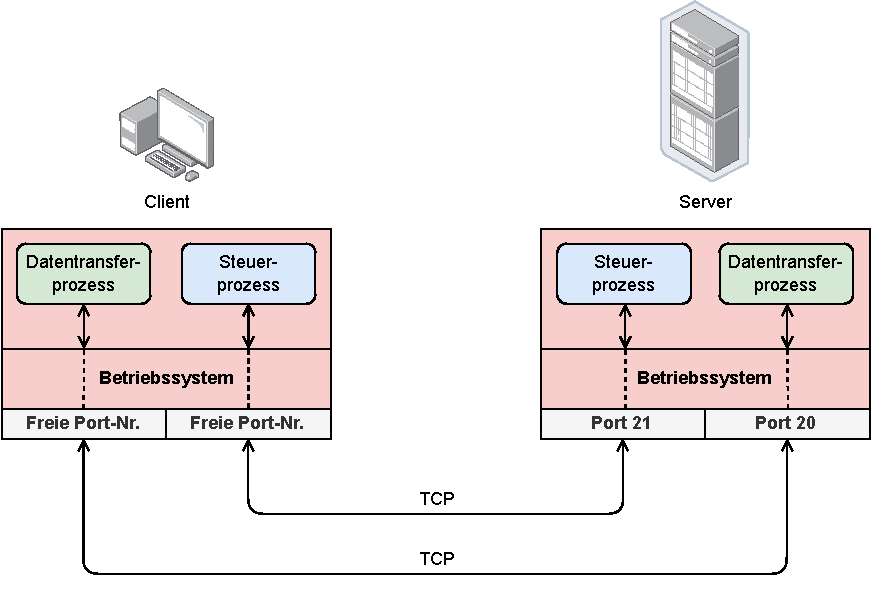
\includegraphics[width=.7\textwidth]{includes/figures/example_ftp.pdf}
\end{example}

\subsection{E-Mail}

\begin{defi}{E-Mail}
    Ein E-Mail-System besteht aus zwei Subsystemen:
    \begin{itemize}
        \item \emph{Mail User Agent (MUA)}:
              \begin{itemize}
                  \item E-Mail-Programm auf dem Client-Rechner des Benutzers
                  \item Empfang und Anzeigen von E-Mails
                  \item Erstellung neuer E-Mails und Beantwortung früherer E-Mails
                  \item Speichern und Verwalten empfangener E-Mails
              \end{itemize}
        \item \emph{Mail Submission Agent (MSA)} bzw. \emph{Message Transfer Agent (MTA)}:
              \begin{itemize}
                  \item Mailserver als langlebiger Prozess
                  \item MSA nimmt E-Mails entgegen, die von MUA losgeschickt wurden und leitet diese ggf. über mehrere MTA (Mail Relays) zum Ziel (\emph{Mail Delivery Agent (MDA)}) weiter
                  \item Zwischenspeicherung von Nachrichten für User oder andere MTA
              \end{itemize}
    \end{itemize}

    \centering
    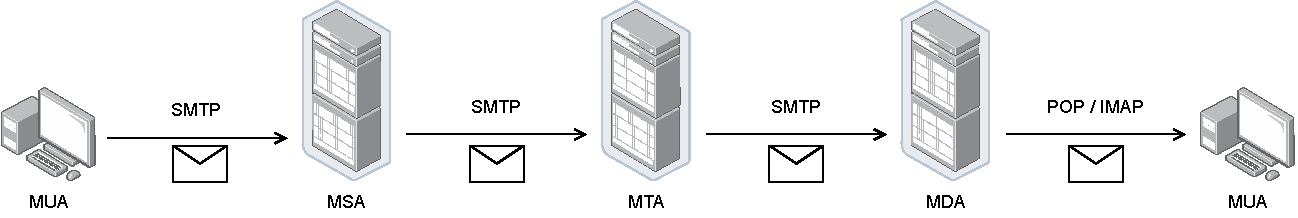
\includegraphics[width=\textwidth]{includes/figures/defi_mail.pdf}
\end{defi}

\begin{bonus}{POP3}
    Das \emph{Post Office Protocol (POP)} ist ein Übertragungsprotokoll, über das ein Client E-Mails von einem E-Mail-Server abholen kann.

    POP3 ist ein ASCII-Protokoll, wobei die Steuerung der Datenübertragung durch Kommandos geschieht, die standardmäßig an den Port 110 geschickt werden.

    POP3 ist in der Funktionalität sehr beschränkt und erlaubt nur das Auflisten, Abholen und Löschen von E-Mails am E-Mail-Server.

    Für weitere Funktionen wie hierarchische Mailboxen direkt am Mailserver, Zugriff auf mehrere Mailboxen während einer Sitzung, Vorselektion der E-Mails usw. müssen Protokolle wie IMAP verwendet werden.
\end{bonus}

\begin{bonus}{SMTP}
    Das \emph{Simple Mail Transfer Protocol (SMTP)}  ist ein Protokoll der Internetprotokollfamilie, das zum Austausch von E-Mails in Computernetzen dient. Es wird dabei vorrangig zum Einspeisen und zum Weiterleiten von E-Mails verwendet. Zum Abholen von Nachrichten kommen andere, spezialisierte Protokolle wie POP3 oder IMAP zum Einsatz.

    SMTP-Server nehmen traditionell Verbindungen auf Port 25 (\texttt{smtp}) entgegen.
\end{bonus}

\begin{bonus}{IMAP}
    Das \emph{Internet Message Access Protocol (IMAP)} ist ein Netzwerkprotokoll, das ein Netzwerkdateisystem für E-Mails bereitstellt.

    IMAP wurde in den 1980er Jahren mit dem Aufkommen von Personal Computern entworfen, um bei der Mail-Kommunikation Abhängigkeiten von einzelnen Client-Rechnern aufzulösen.

    Zu diesem Zweck erweitert IMAP die Funktionen und Verfahren des Post Office Protocol (POP) so, dass Benutzer ihre Mails, Ordnerstrukturen und Einstellungen auf den Servern speichern und belassen können.

    Während bei der Verwendung von POP die Nachrichten entweder nach dem Abruf gelöscht oder beim nächsten Abruf erneut empfangen werden, ermöglicht IMAP eine zentrale Verwaltung mit Suchfunktion und serverseitiger Gelesen-Markierung.
\end{bonus}

\subsection{Verwaltungsprotokolle}

\begin{bonus}{Telnet}
    \emph{Telnet (Teletype Network)} ist ein heutzutage weniger verbreitetes Netzwerkprotokoll.

    Dieses alte und bekannte Client/Server-Protokoll basiert auf einem zeichenorientierten Datenaustausch über eine TCP-Verbindung.

    Telnet wird typischerweise zur Fernsteuerung von Computern in Form von textbasierten Ein- und Ausgaben eingesetzt.
    Hierzu baut der Telnet-Client eine unverschlüsselte Verbindung zu einem Telnet-Server auf.

    In dieser Phase wird ein notwendiges Kennwort im Klartext übergeben.

    Nach dem Verbindungsaufbau wird das Telnet-Protokoll optional initiiert.
    Üblicherweise handelt es sich um eine Login-Konsole mit voller Befehlsgewalt.

    Durch die hohe Befehlsgewalt und die unverschlüsselte Übertragung gilt dieses Verfahren als unsicher und sollte durch eine SSH-Verbindung ersetzt werden, die auch das Telnet-Protokoll umsetzt, aber verschlüsselt überträgt.
\end{bonus}

\begin{defi}{SSH}
    \emph{Secure Shell} oder \emph{SSH} bezeichnet ein kryptographisches Netzwerkprotokoll für den sicheren Betrieb von Netzwerkdiensten über ungesicherte Netzwerke.

    Häufig wird es verwendet, um lokal eine entfernte Kommandozeile verfügbar zu machen, d. h., auf einer lokalen Konsole werden die Ausgaben der entfernten Konsole ausgegeben, und die lokalen Tastatureingaben werden an den entfernten Rechner gesendet.
    Genutzt werden kann dies z. B. zur Fernwartung eines in einem entfernten Rechenzentrum stehenden Servers.

    SSH verwendet die Client–Server-Architektur. Eine SSH-Client-Anwendung verbindet sich also mit einem SSH-Server.

    Anwendungen sind:
    \begin{itemize}
        \item \emph{Secure System Administration} (Sichere Systemverwaltung)
        \item \emph{Secure Application Tunneling} (Sicheres Tunneln)
        \item \emph{Secure Remote Command Execution} (Sichere Ausführung von Kommandos)
    \end{itemize}
\end{defi}

\begin{bonus}{SSH-Tunnel}
    Ein \emph{SSH-Tunnel} ist ein gesicherter Kanal, der Netzwerk-Protokolle einbetten und verschlüsselt übertragen kann. Der Tunnel führt dabei in der Regel von einem Rechner innerhalb eines unsicheren Netzwerks zu einem Server/Netz des Vertrauens.

    Durch diese Form der Portweiterleitung können TCP-Protokolle wie HTTP (Webseiten) oder SMTP (E-Mail) durch ein fremdes Netz (meist das Internet) hindurch gesichert verwendet bzw. überhaupt erst zugänglich gemacht werden.

    Der Aufbaus des Tunnels erfolgt nach folgenden Muster:

    \centering
    \texttt{ssh benutzer@FernerHost -L <lokaler Port>:<Ziel-Host>:<ferner Port>}
\end{bonus}

\begin{bonus}{SNMP}
    Das \emph{Simple Network Management Protocol (SNMP)}  ist ein Netzwerkprotokoll um Netzwerkelemente (z. B. Router, Server, Switches, Drucker, Computer usw.) von einer zentralen Station aus überwachen und steuern zu können.
\end{bonus}